% ============================================================
\section{Elektrische Energiesysteme, Energieformen und Leistungsberechnung}

% ============================================================
\subsection{Grundlagen: Energie und Leistung}

\subsubsection{Definition Energie}

Energie ist die Fähigkeit eines Systems, Arbeit zu verrichten.

Einheit:
\[
[E] = \text{Joule (J)}
\]

1 Joule:
\[
1\,\text{J} = 1\,\text{N}\cdot\text{m}
\]

Weitere gebräuchliche Einheiten:
\[
1\,\text{kWh} = 3{,}6 \cdot 10^6\,\text{J}
\]

\subsubsection{Definition Leistung}

Leistung ist die pro Zeit umgesetzte Energie.

\[
P = \frac{E}{t}
\]

Variablen:
\begin{itemize}
\item $P$ = Leistung [W]
\item $E$ = Energie [J]
\item $t$ = Zeit [s]
\end{itemize}

Einheit:
\[
1\,\text{W} = 1\,\text{J/s}
\]

% ============================================================
\subsection{Mechanische Energieformen}

% ------------------------------------------------------------
\subsubsection{Lageenergie (potentielle Energie)}

\[
E_{pot} = m g h
\]

Variablen:
\begin{itemize}
\item $m$ = Masse [kg]
\item $g$ = Erdbeschleunigung ($9{,}81\,\text{m/s}^2$)
\item $h$ = Höhendifferenz [m]
\end{itemize}

Theorie:
Lageenergie entsteht durch ein Kraftfeld (z.B. Gravitation).  
Sie ist proportional zur Masse und zur Höhenlage.

% ------------------------------------------------------------
\subsubsection{Bewegungsenergie (kinetische Energie)}

\[
E_{kin} = \frac{1}{2} m v^2
\]

Variablen:
\begin{itemize}
\item $m$ = Masse [kg]
\item $v$ = Geschwindigkeit [m/s]
\end{itemize}

Theorie:
Kinetische Energie steigt quadratisch mit der Geschwindigkeit.

% ------------------------------------------------------------
\subsubsection{Rotationsenergie}

\[
E_{rot} = \frac{1}{2} J \omega^2
\]

Variablen:
\begin{itemize}
\item $J$ = Trägheitsmoment [kg m$^2$]
\item $\omega$ = Winkelgeschwindigkeit [rad/s]
\end{itemize}

Zusammenhang:
\[
\omega = 2\pi \frac{n}{60}
\]

\begin{itemize}
\item $n$ = Drehzahl [U/min]
\end{itemize}

Theorie:
Rotierende Massen speichern Energie abhängig von Masseverteilung und Drehzahl.

% ------------------------------------------------------------
\subsubsection{Federenergie}

\[
E_{Feder} = \frac{1}{2} k x^2
\]

Variablen:
\begin{itemize}
\item $k$ = Federkonstante [N/m]
\item $x$ = Auslenkung [m]
\end{itemize}

Theorie:
Elastische Systeme speichern Energie proportional zum Quadrat der Auslenkung.

% ============================================================
\subsection{Thermische Energie}

\subsubsection{Wärmeenergie}

\[
Q = m c \Delta T
\]

Variablen:
\begin{itemize}
\item $m$ = Masse [kg]
\item $c$ = spezifische Wärmekapazität [J/(kgK)]
\item $\Delta T$ = Temperaturdifferenz [K]
\end{itemize}

Theorie:
Wärmeenergie beschreibt die innere Energieänderung durch Temperaturerhöhung.

% ============================================================
\subsection{Elektrische Energie}

% ------------------------------------------------------------
\subsubsection{Elektrische Arbeit}

\[
E = U I t
\]

Variablen:
\begin{itemize}
\item $U$ = Spannung [V]
\item $I$ = Strom [A]
\item $t$ = Zeit [s]
\end{itemize}

% ------------------------------------------------------------
\subsubsection{Kondensatorenergie}

\[
E_C = \frac{1}{2} C U^2
\]

\begin{itemize}
\item $C$ = Kapazität [F]
\item $U$ = Spannung [V]
\end{itemize}

Theorie:
Elektrische Feldenergie im Dielektrikum.

% ------------------------------------------------------------
\subsubsection{Spulenenergie}

\[
E_L = \frac{1}{2} L I^2
\]

\begin{itemize}
\item $L$ = Induktivität [H]
\item $I$ = Strom [A]
\end{itemize}

Theorie:
Magnetische Feldenergie im Induktor.

% ============================================================
\subsection{Mechanische Leistung}

% ------------------------------------------------------------
\subsubsection{Hubleistung}

\[
P = m g v
\]

\begin{itemize}
\item $v$ = Hubgeschwindigkeit [m/s]
\end{itemize}

% ------------------------------------------------------------
\subsubsection{Drehleistung}

\[
P = M \omega
\]

\begin{itemize}
\item $M$ = Drehmoment [Nm]
\item $\omega$ = Winkelgeschwindigkeit [rad/s]
\end{itemize}

% ============================================================
\subsection{Hydraulische Leistung}

\[
P = \rho g Q H
\]

Variablen:
\begin{itemize}
\item $\rho$ = Dichte [kg/m$^3$]
\item $Q$ = Volumenstrom [m$^3$/s]
\item $H$ = Fallhöhe [m]
\end{itemize}

Mit Wirkungsgrad:
\[
P_{el} = \eta \rho g Q H
\]

\begin{itemize}
\item $\eta$ = Wirkungsgrad
\end{itemize}

% ============================================================
\subsection{Wirkungsgrad}

\[
\eta = \frac{P_{ab}}{P_{zu}}
\]

\begin{itemize}
\item $P_{ab}$ = abgegebene Leistung
\item $P_{zu}$ = zugeführte Leistung
\end{itemize}

% ============================================================
\subsection{Drehstromleistung}

\[
P = \sqrt{3} U I \cos\varphi
\]

\begin{itemize}
\item $U$ = verkettete Spannung [V]
\item $I$ = Leiterstrom [A]
\item $\cos\varphi$ = Leistungsfaktor
\end{itemize}

% ============================================================
\subsection{Speicherung elektrischer Energie}

\begin{center}
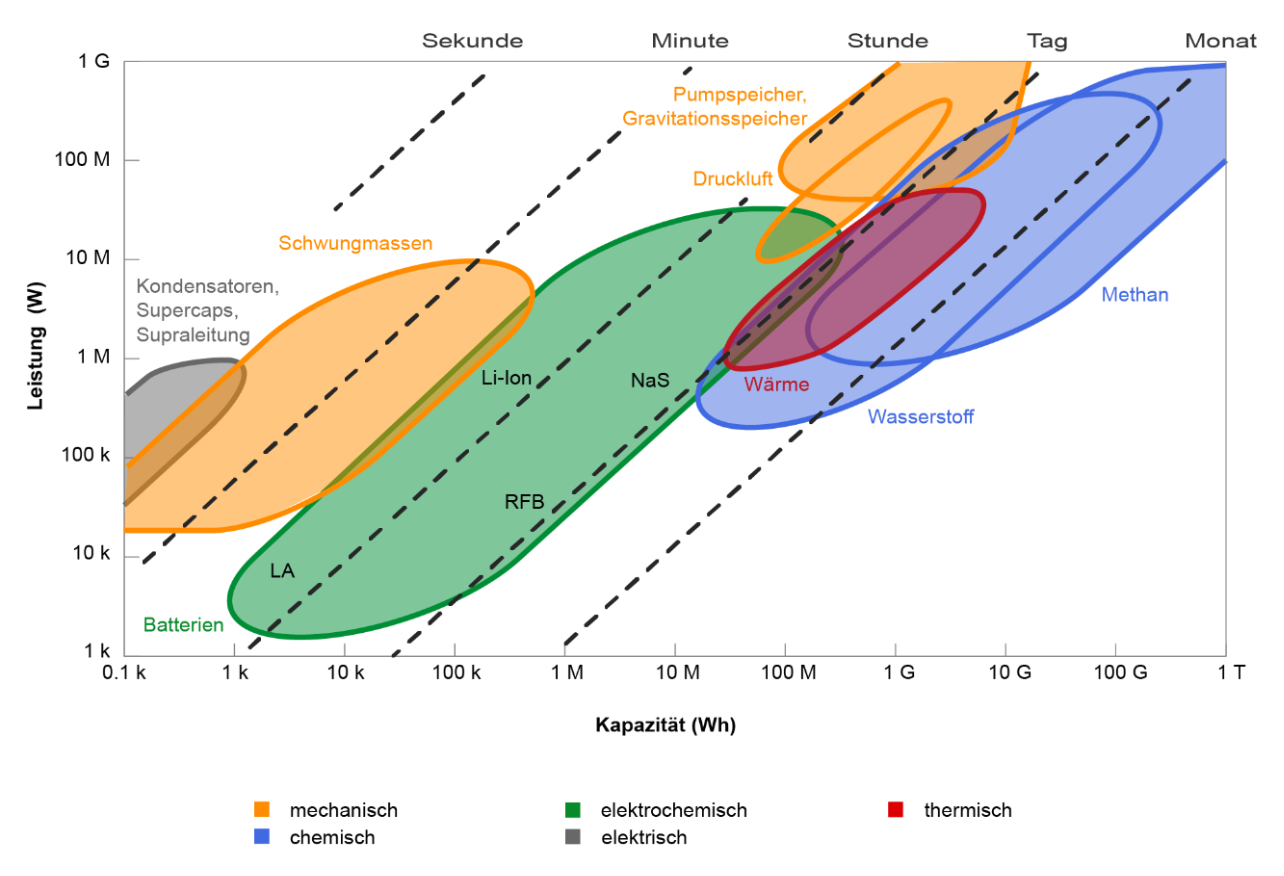
\includegraphics[width=0.8\linewidth]{images/Kapazität_Leistung.png}
\end{center}
\begin{center}
    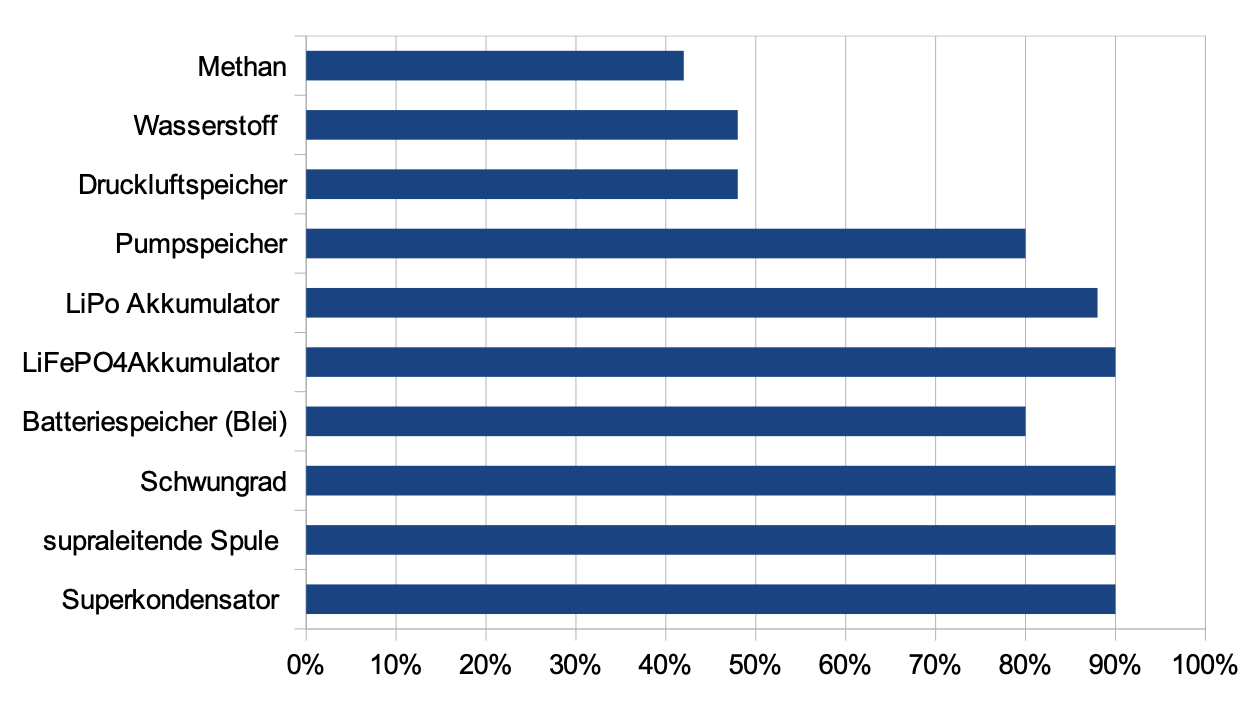
\includegraphics[width=0.8\linewidth]{images/speicher.png}
\end{center}

Allgemein:
\[
E = P t
\]

Beispiel Batterie:
\[
E = U \cdot Ah
\]

Umrechnung:
\[
1\,Ah = 3600\,C
\]

% ============================================================
\subsection{Saisonale Elektrizitätsbilanz und Winterlücke}
\begin{center}
    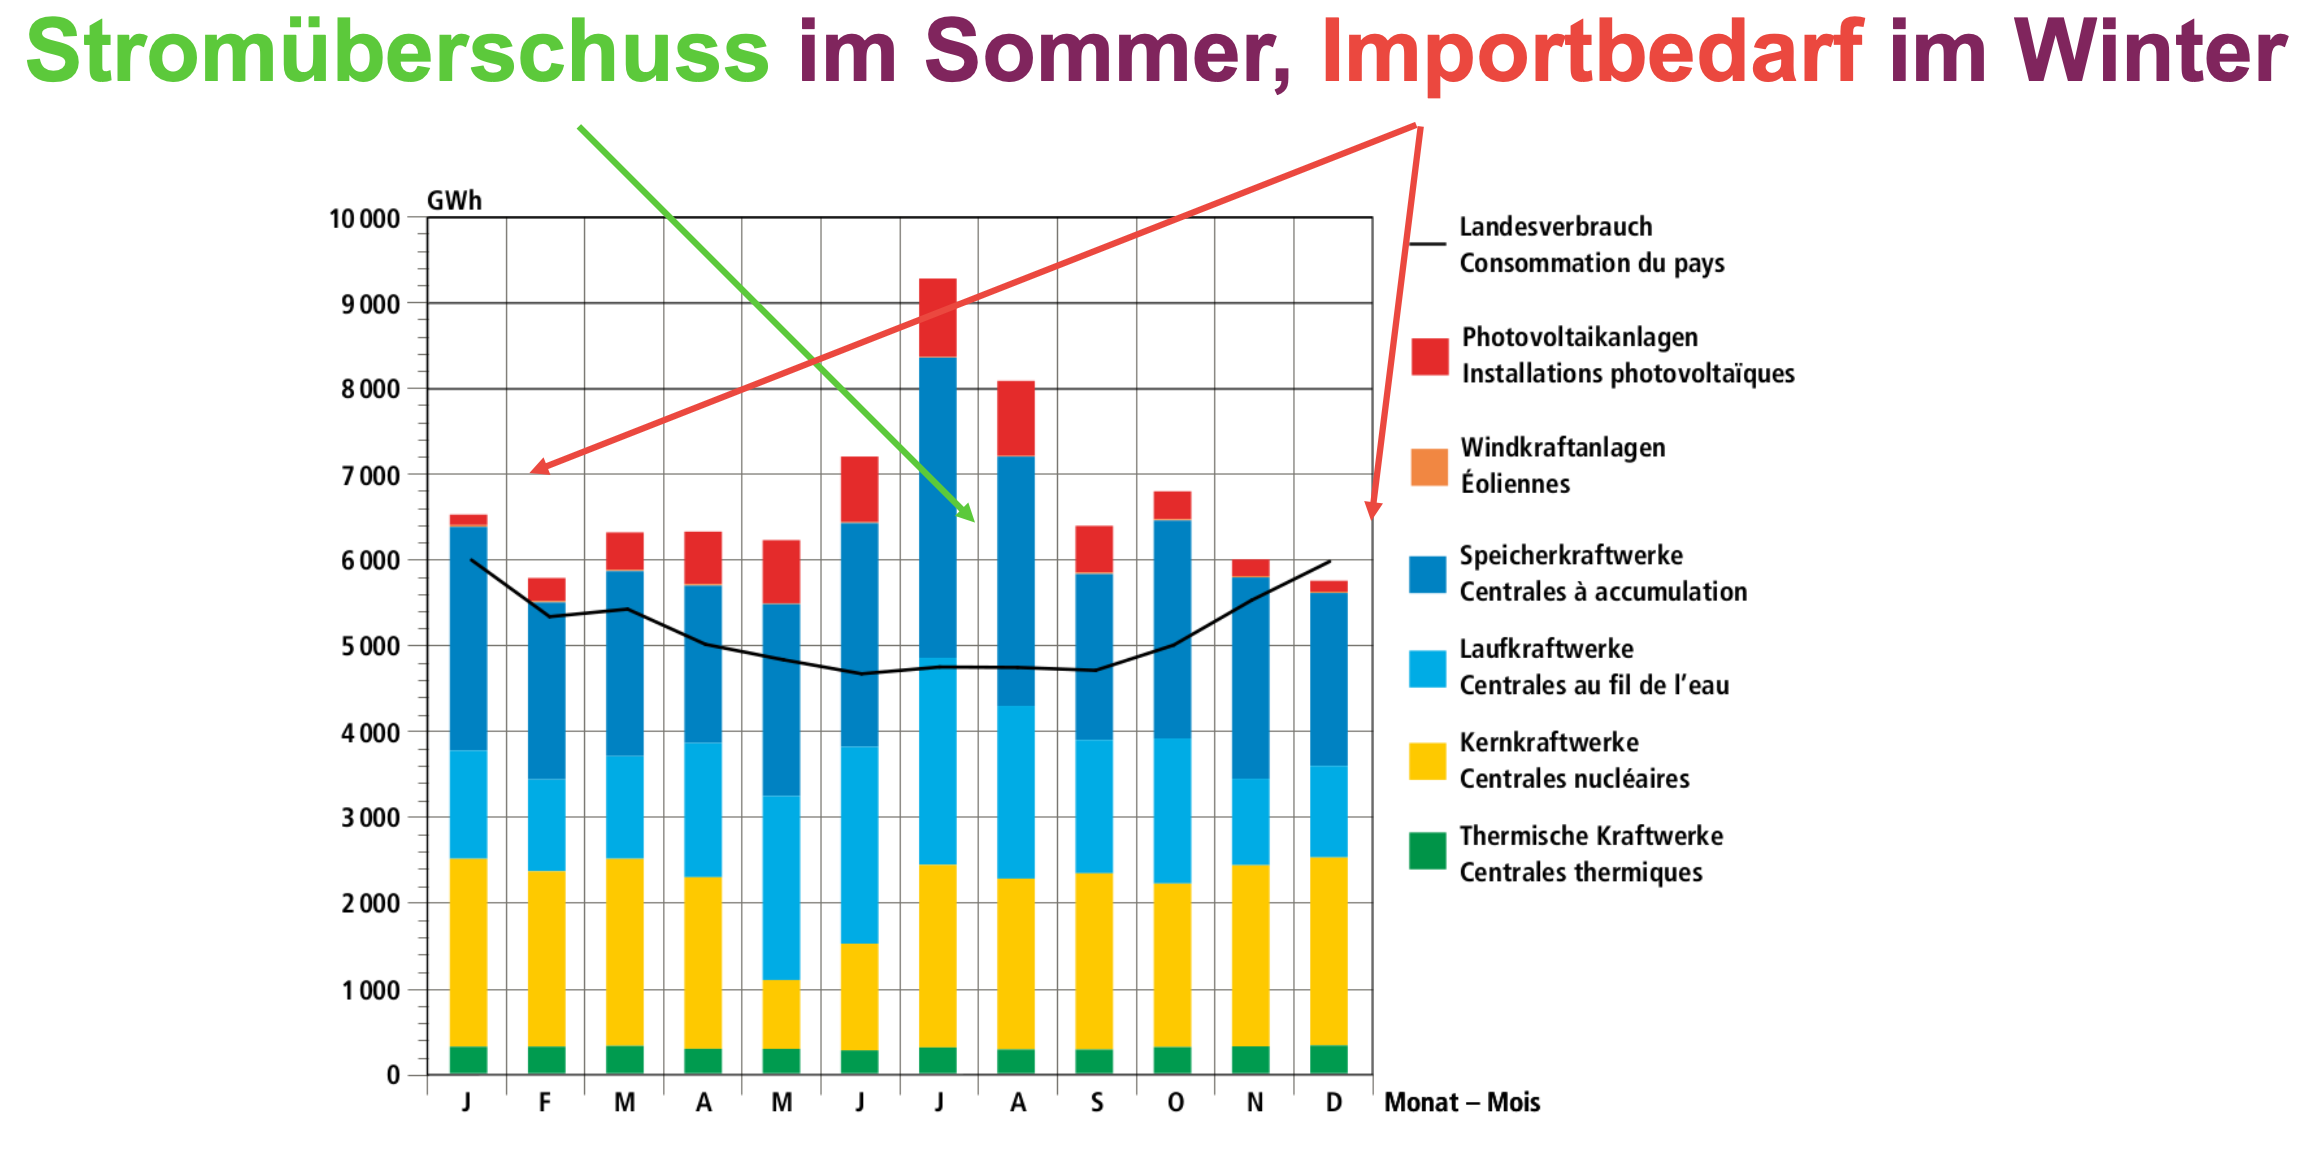
\includegraphics[width=0.8\linewidth]{images/jahresverlauf.png}
\end{center}

\subsubsection{Hydrologisches Jahr}

Definition:
\[
1.\ Oktober \rightarrow 30.\ September
\]

Begründung:
Die Wasserführung der Flüsse folgt hydrologischen Zyklen
(Schneeschmelze, Niederschlag) und nicht dem Kalenderjahr.

\subsubsection{Ganzjahresbilanz}

Grundgleichung:

\[
Erzeugung = Verbrauch + Export - Import
\]

Wichtig:
Eine positive Jahresbilanz bedeutet nicht automatisch
Versorgungssicherheit.

Problem:
Zeitliche Diskrepanz zwischen Erzeugung und Bedarf.

\subsubsection{Sommer- und Wintercharakteristik}

Sommer:

\begin{itemize}
\item Hohe Laufwasserproduktion
\item Hohe PV-Produktion
\item Exportüberschüsse
\end{itemize}

Winter:

\begin{itemize}
\item Geringe PV-Produktion
\item Höherer Verbrauch
\item Importbedarf
\end{itemize}

\subsubsection{Winterlücke}

Definition:
Positiver Importsaldo im Winterhalbjahr.

Ursachen:

\begin{itemize}
\item Saisonale Produktionsverschiebung
\item Begrenzte Speicherkapazität
\item Hohe Last bei tiefen Temperaturen
\end{itemize}

Kritisch:
Mehrwöchige Perioden mit geringer Wind- und Solarproduktion
("kalte Dunkelflaute").

\subsubsection{Rolle der Speicherkraftwerke}

Reservoirs ermöglichen:

\[
E_{Winter} > E_{natürlicher\ Zufluss}
\]

Mechanismus:
Sommerüberschuss → Speicherung → Winterproduktion.

Grenze:
Speicherseen können saisonale Differenz nur teilweise ausgleichen.

% ============================================================
\subsection{Belastungsverlauf und Erzeugungsstruktur}
\begin{center}
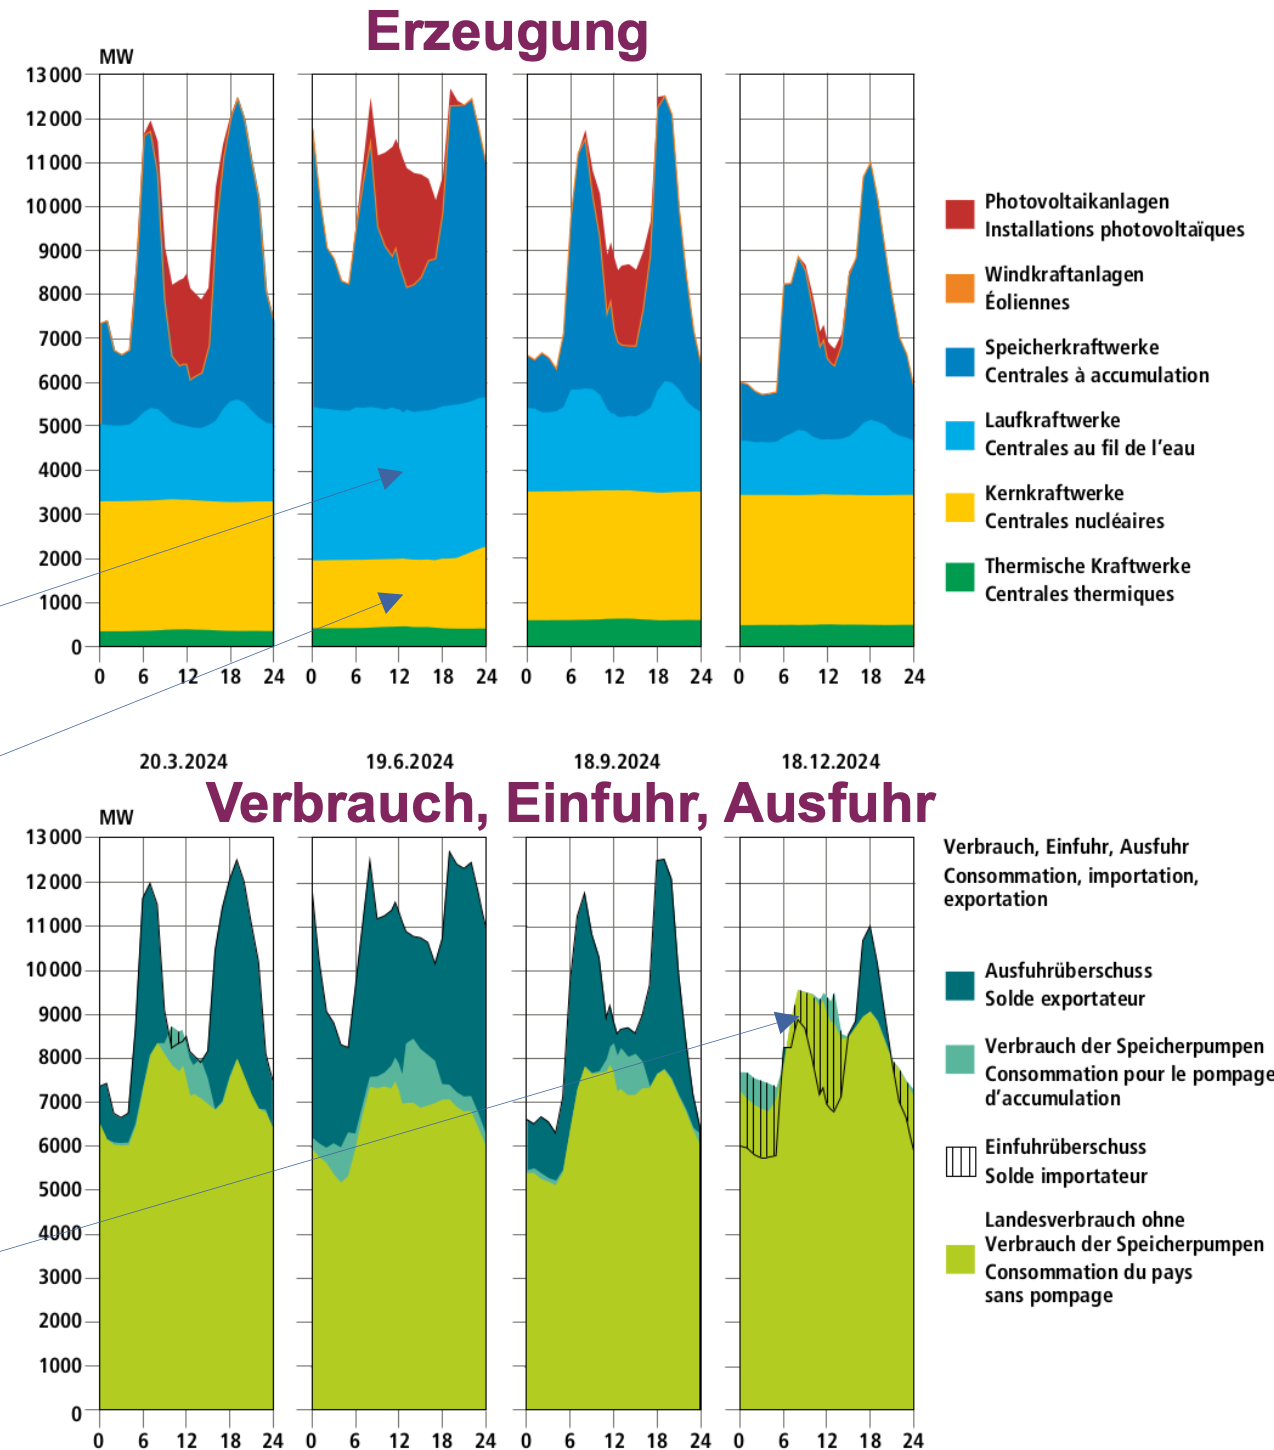
\includegraphics[width=0.8\linewidth]{images/belastungsverlauf.png}
\end{center}

\subsubsection{Grundprinzip Lastverlauf}

Der Stromverbrauch variiert:

\begin{itemize}
\item Tageszeitlich
\item Wochentagsabhängig
\item Saisonabhängig
\end{itemize}

Es gilt jederzeit:

\[
P_{Erzeugung} = P_{Verbrauch} + P_{Export} - P_{Import}
\]

\subsubsection{Typischer Tagesverlauf}

Charakteristika:

\begin{itemize}
\item Morgenanstieg
\item Mittagsplateau
\item Abendspitze
\item Nachttief
\end{itemize}

\subsubsection{Erzeugungscharakteristik nach Technologie}

Kernkraft:

\begin{itemize}
\item Konstante Grundlast
\item Geringe Flexibilität
\end{itemize}

Laufwasserkraft:

\begin{itemize}
\item Abhängig von Wasserführung
\item Im Sommer höher
\end{itemize}

Speicherkraftwerke:

\begin{itemize}
\item Hohe Flexibilität
\item Einsatz in Spitzenlastzeiten
\item Optimierung nach Marktpreisen
\end{itemize}

Photovoltaik:

\begin{itemize}
\item Mittagspeak
\item Starke Winterabsenkung
\end{itemize}

Importe:

\begin{itemize}
\item Vor allem im Winter
\item In „kritischen“ Stunden
\end{itemize}

\subsubsection{Systemische Bedeutung}

Flexibilität wird primär bereitgestellt durch:

\begin{itemize}
\item Speicherkraftwerke
\item Pumpspeicher
\item Internationale Handelsverflechtung
\end{itemize}

\subsubsection{Systematische Einordnung von Speichertechnologien}

Grundprinzip:
Elektrische Energie wird fast immer in andere Energieformen umgewandelt.

Speicherarten:

\begin{itemize}
\item Mechanisch (Pumpspeicher, Schwungrad, Druckluft)
\item Elektrisch (Superkondensator, supraleitende Spule)
\item Chemisch (Batterien, Wasserstoff, Methan)
\end{itemize}

\subsubsection{Pumpspeicher als Referenztechnologie}

Eigenschaften:

\begin{itemize}
\item Hohe Leistung
\item Hohe Speicherkapazität
\item Hoher Wirkungsgrad (70--85\%)
\item Geeignet für saisonale Verschiebung
\end{itemize}

Nettoenergie bei Pumpspeicher:

\[
E_{netto} = E_{Turbine} - E_{Pumpe}
\]

Saisonale Bedeutung:
Reservoirs ermöglichen Winterstromproduktion durch im Sommer gespeichertes Wasser.

% ============================================================
\subsection{Struktur elektrischer Energiesysteme}

\begin{center}
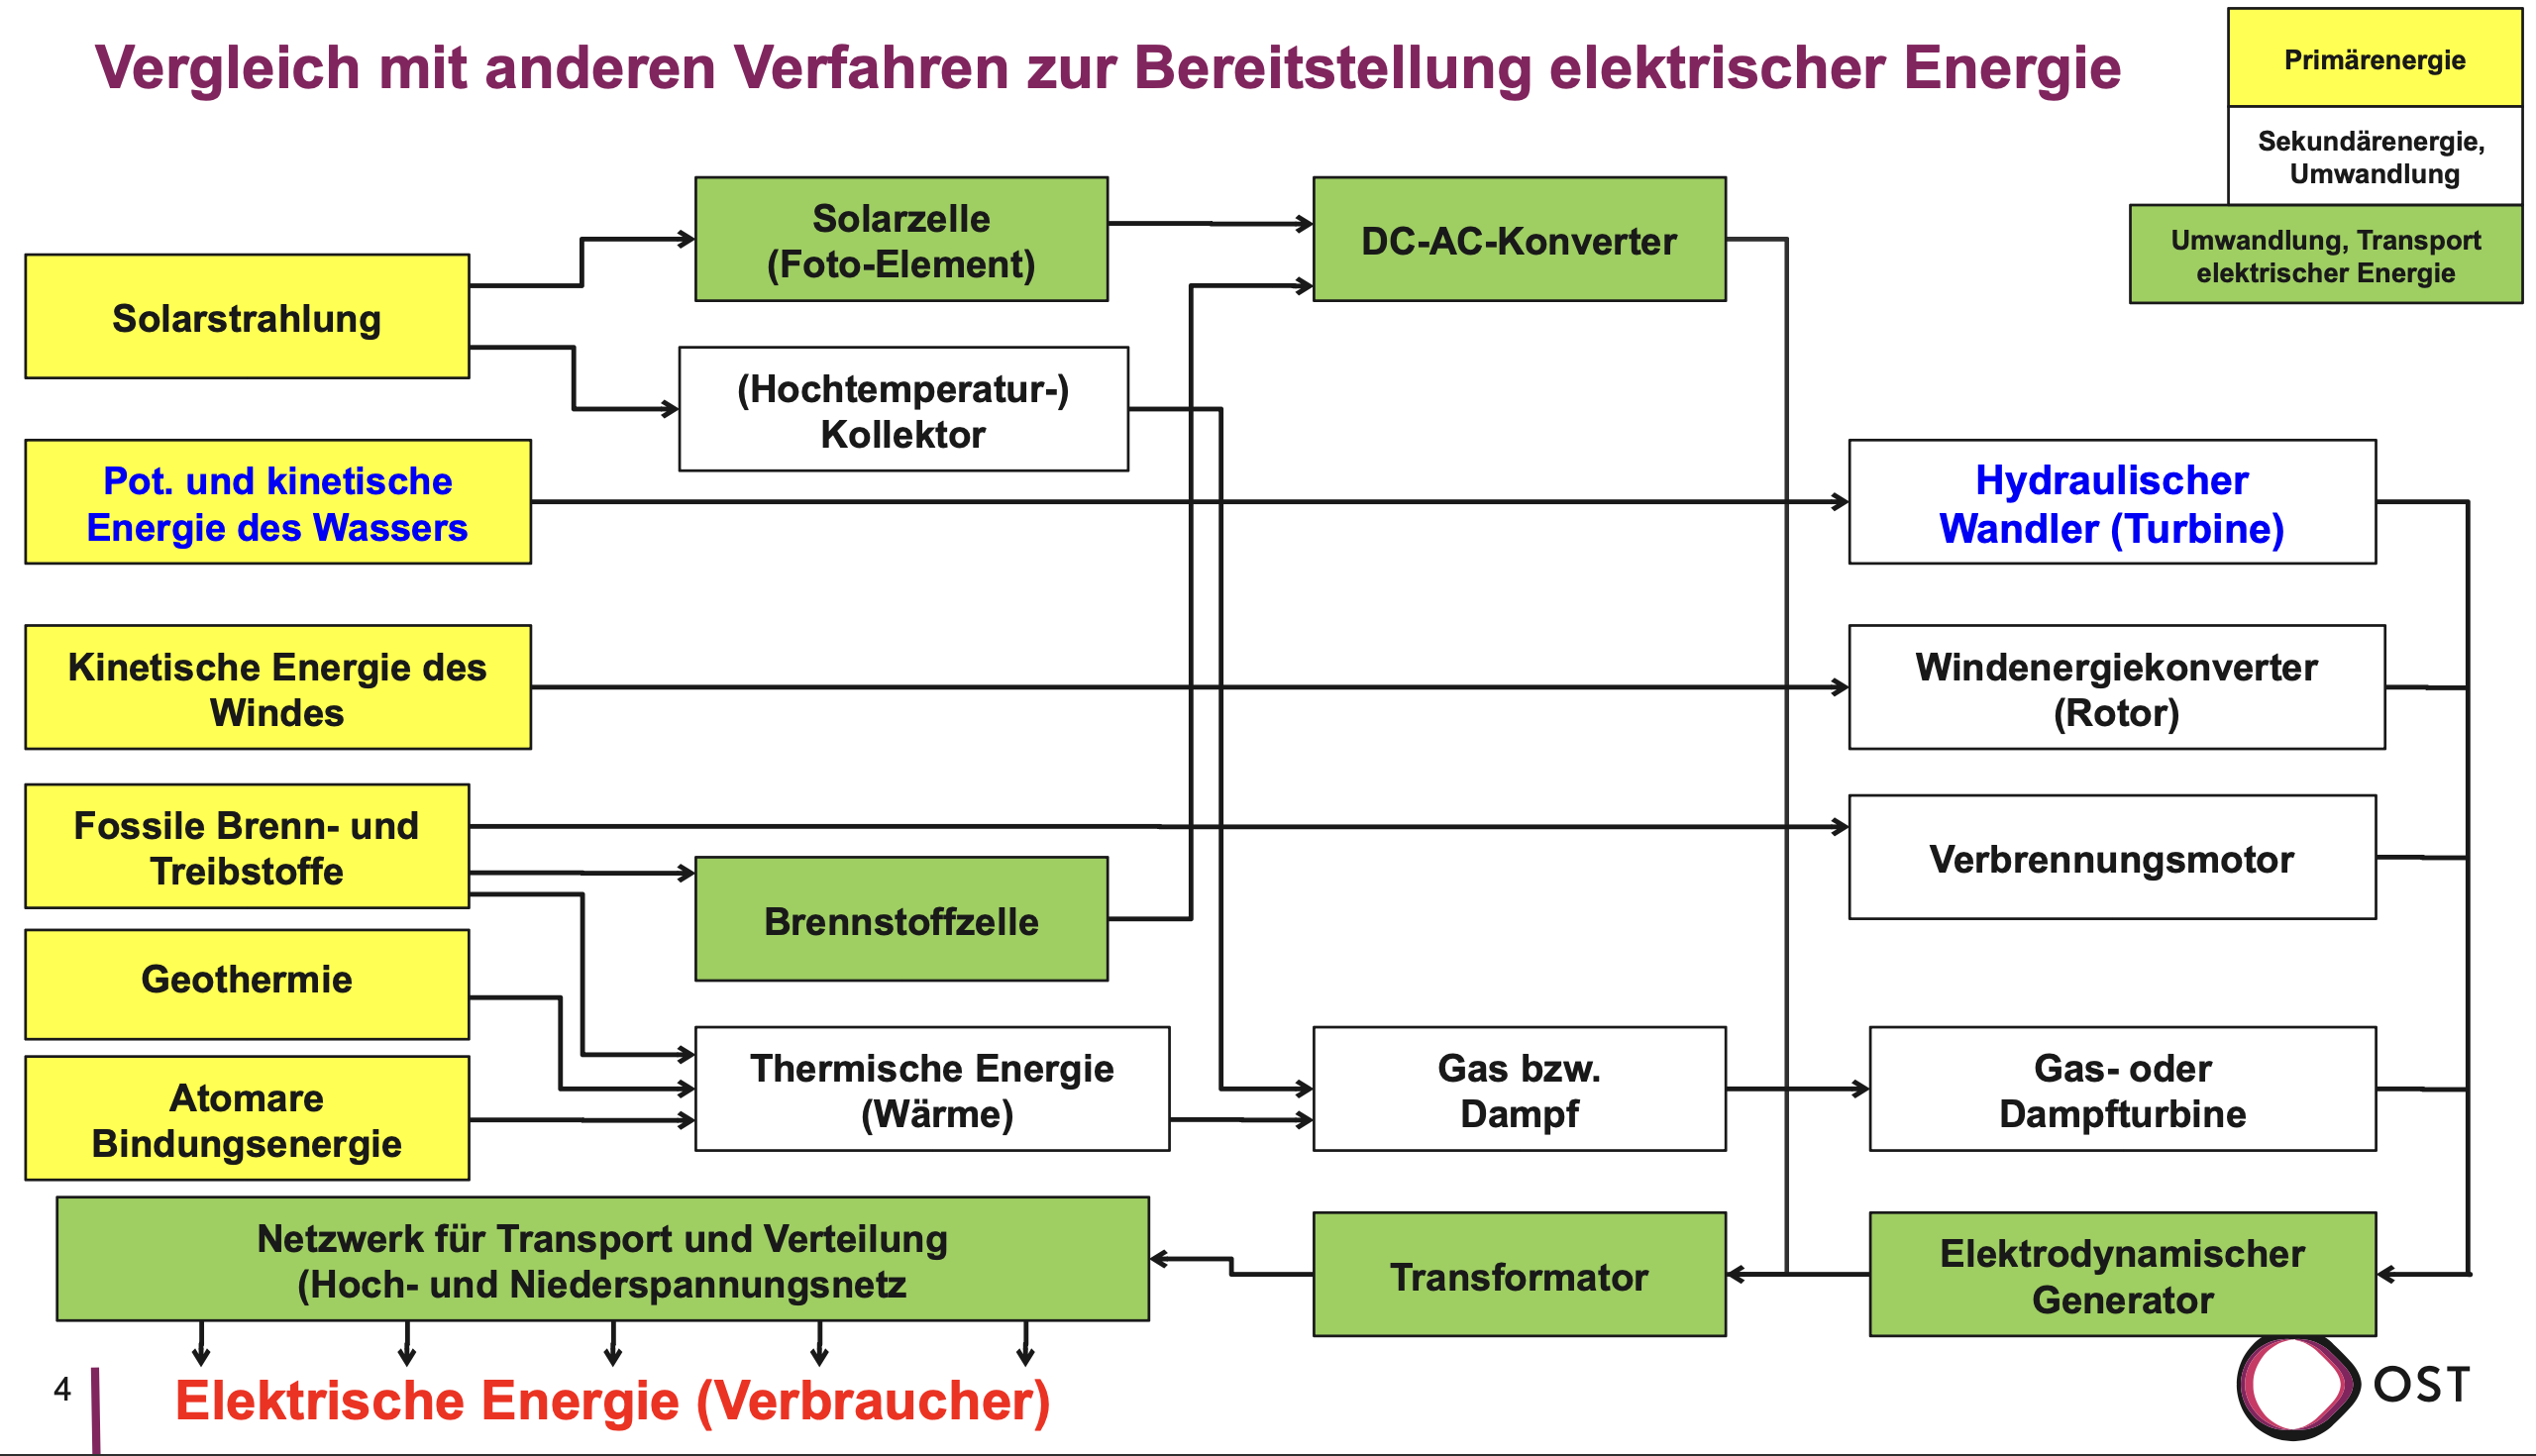
\includegraphics[width=0.8\linewidth]{images/Energie.png}
\end{center}

Bestandteile:
\begin{itemize}
\item Erzeugung
\item Transport
\item Verteilung
\item Verbrauch
\end{itemize}

Leistungsbilanz:
\[
P_{Erzeugung} = P_{Verbrauch} + P_{Export} - P_{Import}
\]

Systemanforderung:
Momentanes Gleichgewicht von Erzeugung und Verbrauch.

% ============================================================
\subsection{Elektrischer Strom als Energieträger}

Elektrische Energiesysteme sind Anlagen, Maschinen und Organisationsformen,
die der Erzeugung, dem Transport und der Verteilung elektrischer Energie dienen.

\subsubsection{Charakteristika elektrischer Energie}

Vorteile:

\begin{itemize}
\item Leicht transportierbar (leitungsgebunden)
\item Spannung transformierbar → verlustarmer Transport
\item Einfach zu verteilen
\item Beliebig dosierbar
\item Sehr gut regelbar
\item Saubere Anwendung beim Endverbraucher
\item Kein Speicher beim Kunden erforderlich
\end{itemize}

Herausforderungen:

\begin{itemize}
\item Gleichzeitigkeit von Erzeugung und Verbrauch
\item Netz als zentrales Infrastrukturelement
\item 40--70\% der Investitionen entfallen auf das Netz
\item Versorgungssicherheit und Netzstabilität
\end{itemize}

\subsubsection{Primär- und Sekundärenergie}

Primärenergie:
Natürlich vorkommende Energiequellen (Wasser, Wind, Sonne, fossile Brennstoffe, Kernenergie).

Sekundärenergie:
Durch Umwandlung erzeugte Energieformen (Elektrizität, Benzin, Fernwärme).

Elektrizität ist Sekundärenergie mit hoher Umwandlungsflexibilität.

% ============================================================
\subsection{Energiewirtschaftliche Marktstruktur}
\begin{center}
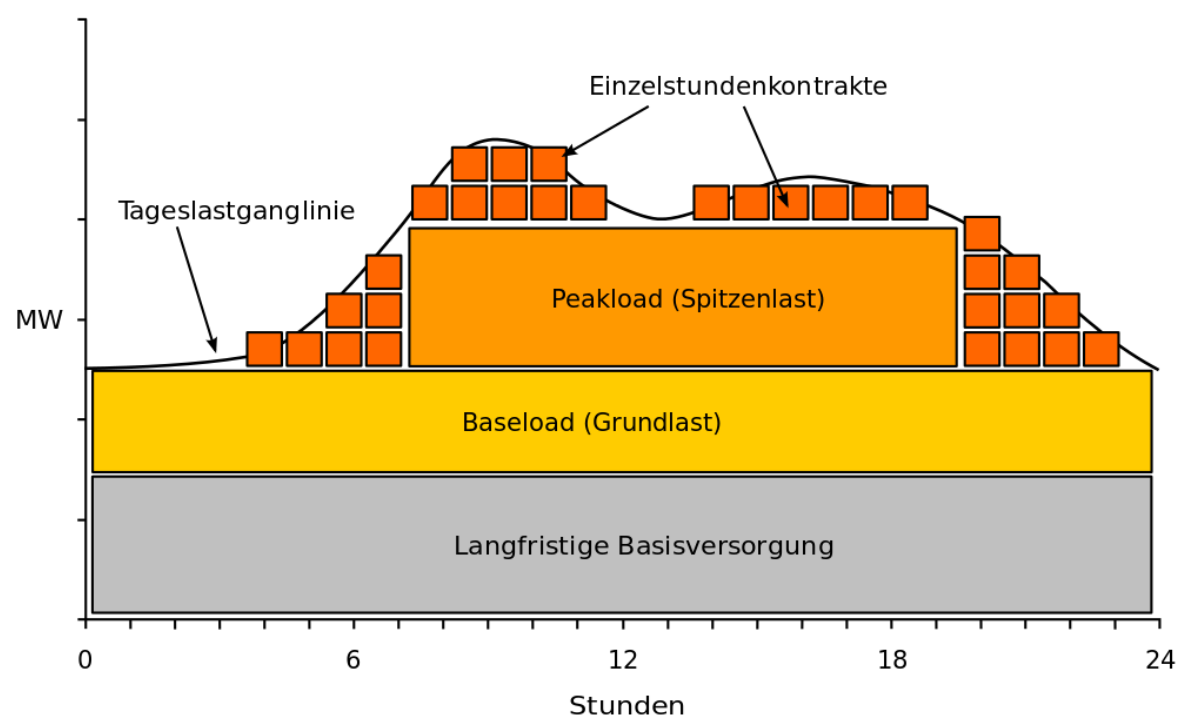
\includegraphics[width=0.8\linewidth]{images/Energiewirtschaft.png}
\end{center}

Baseload:
Konstante Lieferung über 24h.

Peakload:
Lieferung während Hochlaststunden.

Langfristige Basisversorgung:
Investitionsgetriebene Kapazitätsbereitstellung.

Kurzfristige Märkte:
Preisgetriebene Optimierung.

% ============================================================
\subsection{Strommarkt und Merit-Order}

Marktsegmente:
\begin{itemize}
\item Day-Ahead
\item Intraday
\item Terminmarkt
\item Reserveenergie
\end{itemize}

Merit-Order:
Sortierung nach Grenzkosten.

Marktpreis:
\[
p^* = \text{Grenzkosten des marginalen Kraftwerks}
\]

Deckungsbeitrag:
\[
DB = p^* - K_v
\]

\begin{itemize}
\item $K_v$ = variable Kosten
\end{itemize}

\subsubsection{Merit-Order-Effekt durch erneuerbare Energien}

Mechanismus:

\begin{itemize}
\item Wind und PV mit sehr niedrigen Grenzkosten
\item Verschiebung der Angebotskurve nach rechts
\item Marktpreis sinkt
\item Teure Kraftwerke werden verdrängt
\item Deckungsbeiträge sinken
\end{itemize}

Folge:
"Preiskannibalisierung"

Im Extremfall:
Negative Strompreise.

Langfristige Konsequenz:
Diskussion über Kapazitätsmärkte.

\subsubsection{Residualnachfrage}

Die für die Preisbildung relevante Nachfrage ist die
Residualnachfrage:

\[
L_{res} = L_{gesamt} - E_{Wind} - E_{PV}
\]

\begin{itemize}
\item $L_{res}$ = durch konventionelle Kraftwerke zu deckende Last
\item $L_{gesamt}$ = gesamte Netzlast
\item $E_{Wind}, E_{PV}$ = Einspeisung erneuerbarer Energien
\end{itemize}

Der Marktpreis ergibt sich aus den Grenzkosten
des Kraftwerks, das die Residualnachfrage deckt.

\subsubsection{Extremsituationen}

Dunkelflaute:

\[
E_{Wind} \approx 0, \quad E_{PV} \approx 0
\]

Folge:
Maximale thermische Erzeugung erforderlich.

Der Marktpreis wird durch das teuerste noch benötigte
Kraftwerk bestimmt.

Bei Kapazitätsknappheit sind sehr hohe oder negative
Preise möglich.

% ============================================================
\subsection{Investitionsrechnung}

Annuitätsfaktor:
\[
a = \frac{i(1+i)^n}{(1+i)^n - 1}
\]

\begin{itemize}
\item $i$ = Zinssatz
\item $n$ = Nutzungsdauer
\end{itemize}

Jährliche Kapitalkosten:
\[
K_{Kap} = I a
\]

\begin{itemize}
\item $I$ = Investitionssumme
\end{itemize}

Gesamtkosten:
\[
K_{ges} = K_f + K_v
\]

Gewinn:
\[
G = Erlös - K_{ges}
\]

\subsection{Kostenstruktur von Kraftwerken}

Fixe Kosten:

\begin{itemize}
\item Zinsen
\item Amortisation
\item Personal
\item Fixer Unterhalt
\end{itemize}

Variable Kosten:

\begin{itemize}
\item Brennstoff
\item CO$_2$-Zertifikate
\item Betriebsabhängiger Unterhalt
\end{itemize}

Deckungsbeitrag:

\[
DB = Erlös - K_v
\]

Gewinn:

\[
G = DB - K_f
\]

Wichtig:
Einnahmen aus Stromhandel müssen langfristig
die Vollkosten decken.

% ============================================================
\subsection{Zusammenfassung}

Alle Energieformen lassen sich auf folgende Grundprinzipien zurückführen:

\begin{itemize}
\item Energieerhaltung
\item Umwandlung mit Wirkungsgradverlust
\item Leistung als zeitliche Änderungsrate
\item Marktpreisbildung über Grenzkosten
\item Investitionen über Kapitalbindung
\end{itemize}

Damit sind sämtliche Energie- und Leistungsaufgaben vollständig abgedeckt.